\documentclass[]{article}

%%%%%%%%%%%%%%%%%  << MATLAB INCLUSION>>  %%%%%%%%%%%%%%%%%
\usepackage[numbered framed]{mcode}
% Need mcode.sty in current directory
%%%%%%%%%%%%%%%%%  << MATLAB INCLUSION>>  %%%%%%%%%%%%%%%%%

%%%%%%%%%%%%%%%%%  << IMAGE INCLUSION>>  %%%%%%%%%%%%%%%%%
\usepackage{graphicx}
%%%%%%%%%%%%%%%%%  << IMAGE INCLUSION>>  %%%%%%%%%%%%%%%%%
\usepackage{color}
\usepackage{cleveref}
\usepackage{amsmath}
\usepackage{graphicx}
\usepackage{color}
% Other packages
%\usepackage{times, rawfonts, geometry}
%\usepackage{amsmath,amssymb}
%\usepackage{float}

% New commands
\newcommand{\ignore}[1]{}  % {} empty inside = %% comment

% Scientific notation:
\providecommand{\e}[1]{\ensuremath{\times 10^{#1}}}

% General
\newcommand{\parens} [1] {\left(  #1  \right)}
\newcommand{\brackets} [1] {\left[ #1 \right]}
\newcommand{\rootdir}{./Figures/}

% Array
\newcommand{\arrayp}[2]{\parens{ \begin{array}{#1}  #2 \end{array} } }
\newcommand{\arrayb}[2]{\brackets{ \begin{array}{#1}  #2 \end{array} } }

\begin{document}

\title{ASEN 5070-Stastistical Orbit Determination-HW 10}
\author{Zach Dischner}
\date{11-29-2012}
\maketitle


%%%%%%%%%%%%%%%%%%%%%%  << 1 >>  %%%%%%%%%%%%%%%%%%%%%%%%
\section{Problem 1 -Perform Givens Square Root Free Algorithm} 
The Givens Square Root Free Algorithm is, like the Potter and Joseph Algorithms, an alternate method for calculating the covariance matrix, \emph{P}. Its main advantage is that it yields a positive semi-definite covariance matrix, but without the need for computationally expensive square roots. 

In this assignment, I performed the Givens algorithm on the system from homework assignment 8, for a range of $\delta$ values. 

\begin{equation}
	\left[ \begin{array}{c}
		y_1			\\
		y_2			\\
	\end{array}\right]
	=
	\left[ \begin{array}{c}
		3		\\
		2		\\
	\end{array}\right]
	=
	\left[ \begin{array}{cc}
		1	&	\delta	\\
		1	&	1		\\
	\end{array}\right]
	\left[ \begin{array}{c}
		x_1		\\
		x_2		\\
	\end{array}\right]
	+
	\left[ \begin{array}{c}
		\epsilon_1		\\
		\epsilon_2		\\
	\end{array}\right]
\end{equation}


\begin{equation}
	\bar{X}
	=
	\left[ \begin{array}{c}
		\bar{x}_1			\\
		\bar{x}_2			\\
	\end{array}\right]
	=
	\left[ \begin{array}{c}
		4			\\
		7			\\
	\end{array}\right]
\end{equation}


\begin{equation}
	P_0
	=
	\left[ \begin{array}{cc}
		1/\delta^2		&		1			\\
		1			&	1/\delta^2			\\
	\end{array}\right]
\end{equation}


\begin{equation}
	R = I
\end{equation}

\begin{equation}
	\delta = 1x10^{-2}...1x10^{-16}
\end{equation}

For each $\delta$, I calculated $P_2$ and $X_{hat}$. So see how the algorithm performed, I plotted the difference in traces of the Givens result for $P_2$ and the exact solution for $P_2$, found using EQ 4.7.24 in the book. 

\begin{figure}
    \includegraphics[width=5.8in,height=6in]{../Figures/1.png}
    \caption{Truth-State for Different Algorithms}
    \label{fig:State}
\end{figure}

\vspace{5in}
The figure looks like noise, which indicates that the difference in $P_2$ traces is negligible. It falls into the range of computational precision. Compared with some of the other algorithms investigated, the Givens algorithm appears less subject to numerical errors.

Intuitively, I would have assumed this algorithm would not be the ideal choice for calculating $P_2$. It seems that there are so many computations, and any issues from numerical precision errors would be amplified. Avoiding square roots by using these complicated algorithms seems to be an inefficient method, but apparently it works quite well. 




%%%%%%%%%%%%%%%%%%%%%%  << 1 >>  %%%%%%%%%%%%%%%%%%%%%%%%
\section{Problem2-Computational Comparison} 

Next, I verified that the $\sum{e_i^2}$ calculated within the Givens computation matches with the result from the book, EQ 5.4.33. This was done in Matlab, and the result is indeed identical. 


\begin{lstlisting}
	Accumulated e^2 is  :     0.006513006241065
	EQ 5.4.33  sum e^2  :     0.006513006241065
\end{lstlisting}


The code for both of these sections is provided in the following Appendix. 






\vspace{6in}
\appendix{\centerline{\LARGE \bf{Appendix A- MATLAB Generation Code}}}
% This LaTeX was auto-generated from an M-file by MATLAB.
% To make changes, update the M-file and republish this document.

\sloppy
\definecolor{lightgray}{gray}{0.5}
\setlength{\parindent}{0pt}

    
    
\subsection*{Contents}

\begin{itemize}
\setlength{\itemsep}{-1ex}
   \item 1 - Find X, P using Givens and compare.
   \item 2 - Do The Amazing Thing
\end{itemize}
\begin{verbatim}
%%%%%%%%%%%%%%%%%%%%%%%%%%%%%%%%%%%%%%%%%%%%%%%%%%%%%%%%%%%%%%%%%%%%%%%%
%
%
% Zach Dischner-10/31/2012
%
% ASEN 5070-Statistical Orbit Determination
%
% Homework 10
%
% Inputs    : None
%
% Outputs   : Plots for homework 10
%
%
%%%%%%%%%%%%%%%%%%%%%%%%%%%%%%%%%%%%%%%%%%%%%%%%%%%%%%%%%%%%%%%%%%%%%%%%

clc;clear all;close all; format compact;format long g;tic
\end{verbatim}


\subsection*{1 - Find X, P using Givens and compare.}

\begin{verbatim}
e = logspace(-16,-2,1000);

P_Givens    = zeros(2,2,length(e));
P_True      = P_Givens;
X_Givens    = zeros(2,length(e));
tr_Givens   = zeros(length(e),1);
tr_True     = zeros(length(e),1);


Sum_e_squared = zeros(length(e),1);
Sum_e_squared_New = Sum_e_squared;

% Go get plot numbers for the state
for ii = 1:length(e)
    [P_Givens(:,:,ii),X_Givens(:,ii), P_True(:,:,ii),Sum_e_squared(ii),Sum_e_squared_New(ii)] = FindGivens(e(ii));
    tr_Givens(ii)   = trace(P_Givens(:,:,ii));
    tr_True(ii)     = trace(P_True(:,:,ii));
end

% Plot difference in P traces
figure
semilogx(e,abs(tr_Givens - tr_True));
xlabel('\epsilon');ylabel('abs( P Givens - P Batch)'); title('Givens - Batch')
\end{verbatim}

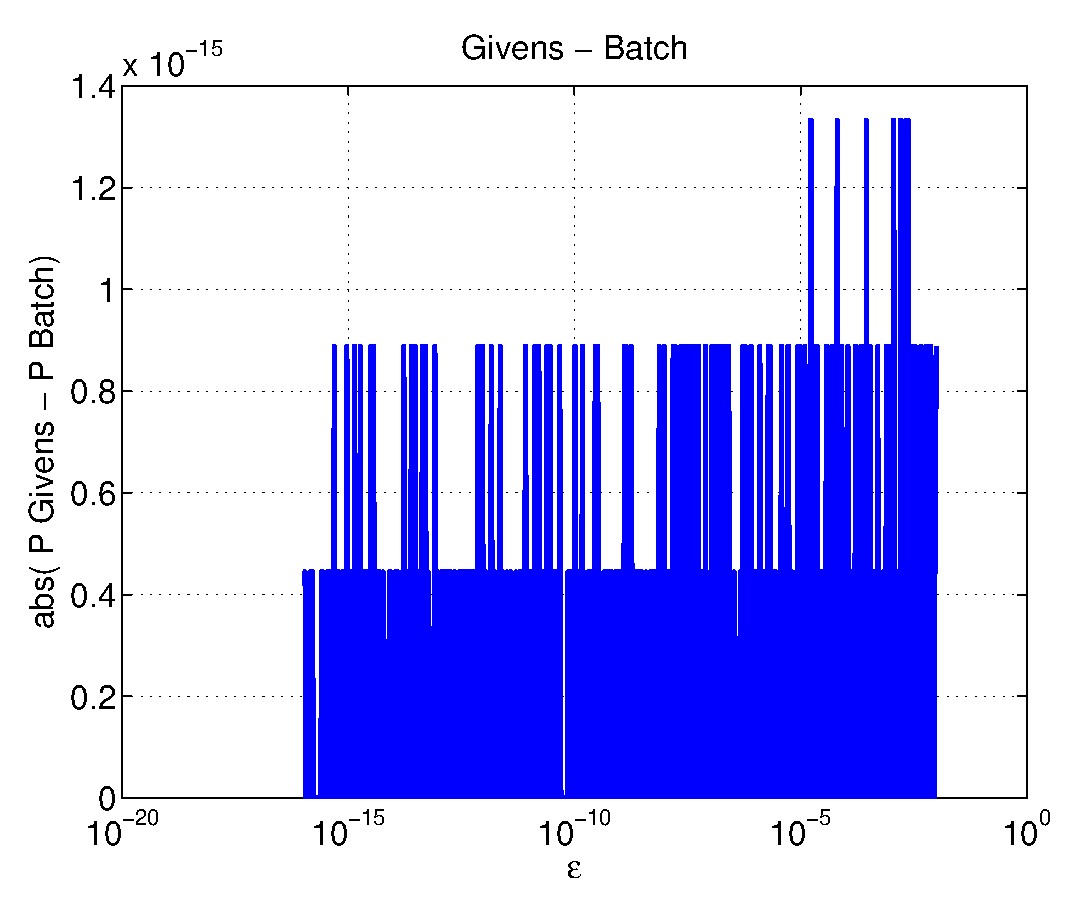
\includegraphics [width=4in]{../html/HW10_01.eps}


\subsection*{2 - Do The Amazing Thing}

\begin{par}
5.4.33 says    sum e\^{}2 = Eta\_hat' * Rbar' * Rbar * Eta\_hat +  sum(/epsilon\^{}2) Eta\_hat = xhat - xbar /epsilon = yi-Hi*xhat
\end{par} \vspace{1em}
\begin{verbatim}
delta = 1e-2;

Rbar    = eye(2,2);
Xbar    = [4;7];
H       = [1 delta;1 1];
y1      = 3;
y2      = 2;

% Xhat = X_Givens(:,1);
[p,Xhat,p2,Sum_e_squared,Sum_e_squared_New]=FindGivens(1e-2);

Eta_hat = Xhat - Xbar;

fprintf('Accumulated e^2 is  :     %3.15f\n\n',Sum_e_squared)

fprintf('EQ 5.4.33  sum e^2  :     %3.15f\n\n',Sum_e_squared_New)

% Make figures awesome and save
figure_awesome('save')
\end{verbatim}

        \color{lightgray} \begin{verbatim}Accumulated e^2 is  :     0.006513006241065

EQ 5.4.33  sum e^2  :     0.006513006241065

\end{verbatim} \color{black}
    
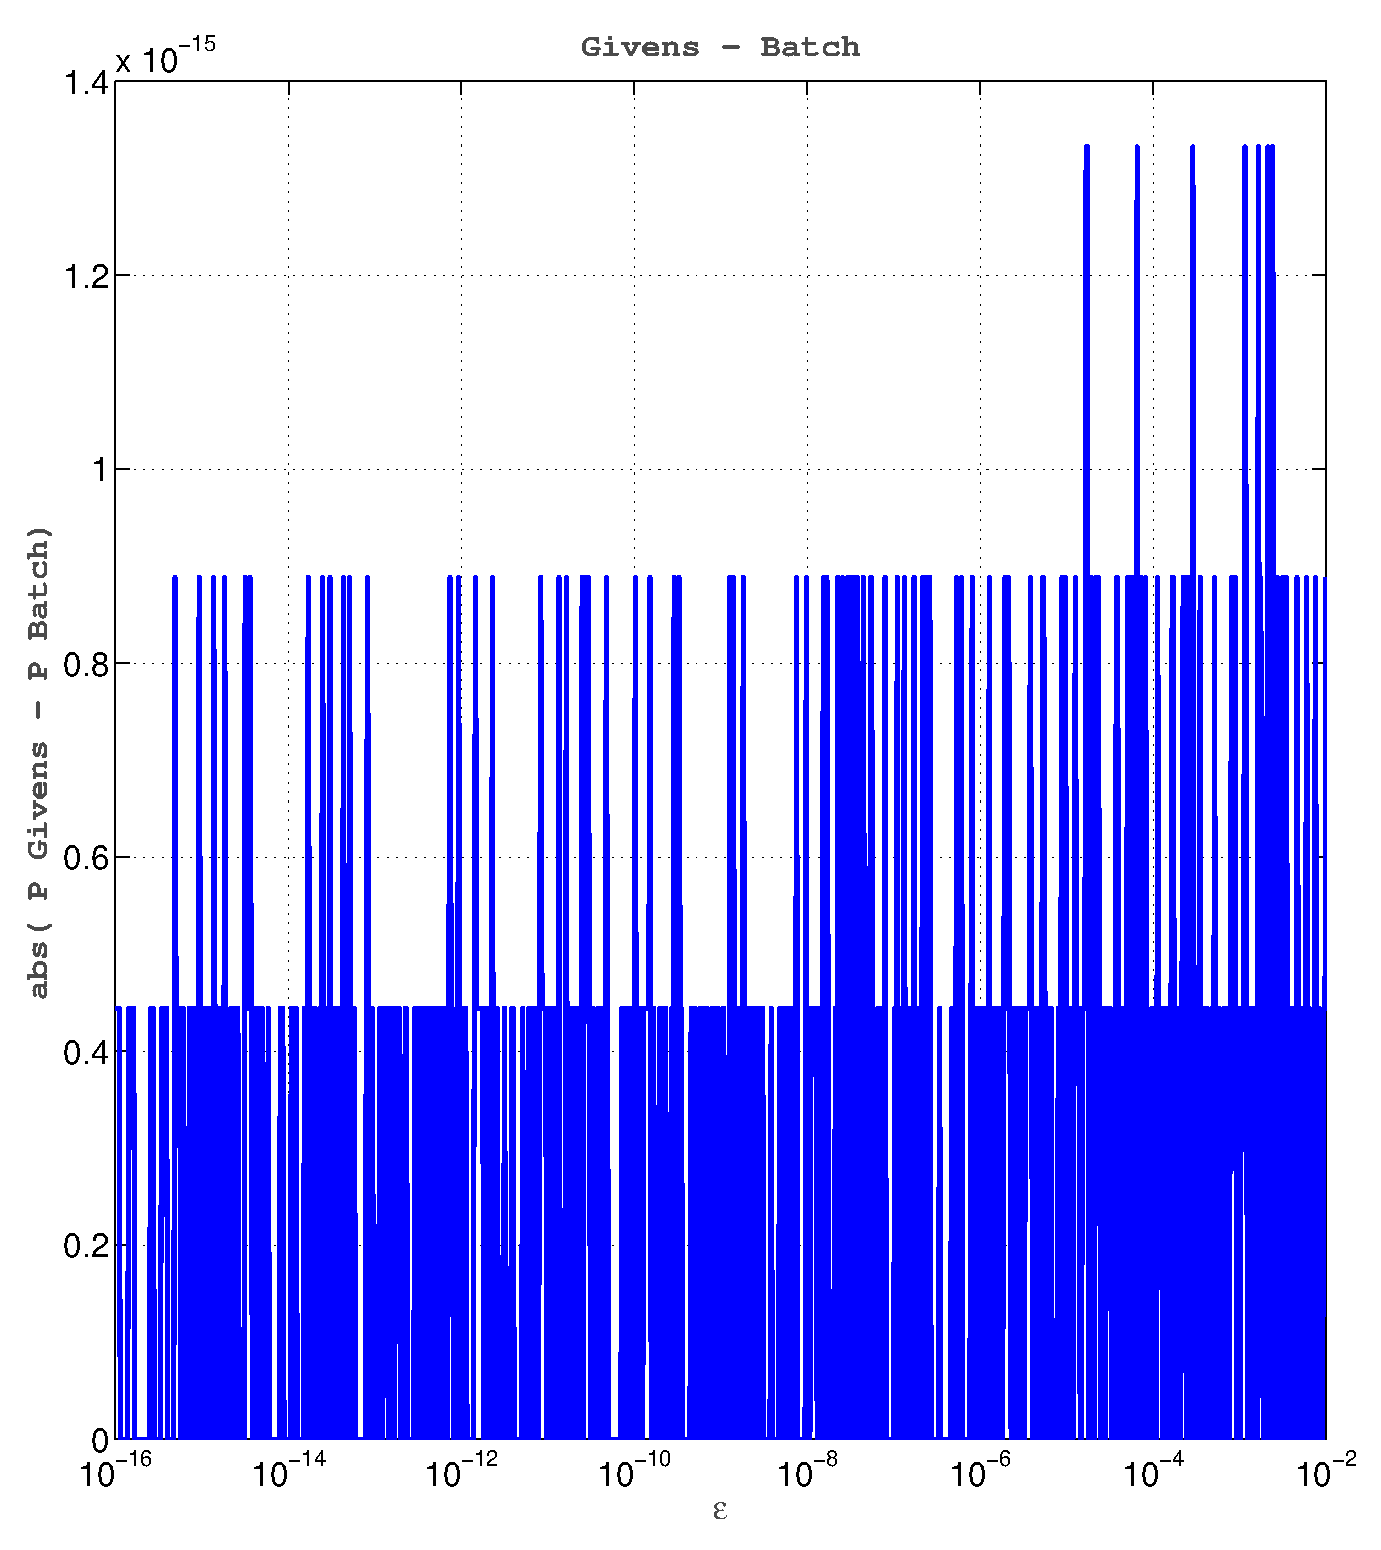
\includegraphics [width=4in]{../html/HW10_02.eps}



\end{document}
    










\end{document}